A jelen dolgozatban egy árakat figyelő alkalmazás készítéséről van szó, mellyel különböző termékek árát lehet követni, bizonyos webshopokon. Az alkalmazás több platformon is elérhető, hogy minél könnyebben eljusson a kívánt információ a felhasználóig. A következőkben tárgyalva lesznek a felhasználói, valamint rendszer követelmények is.

\begin{figure}[H]
    \centering
    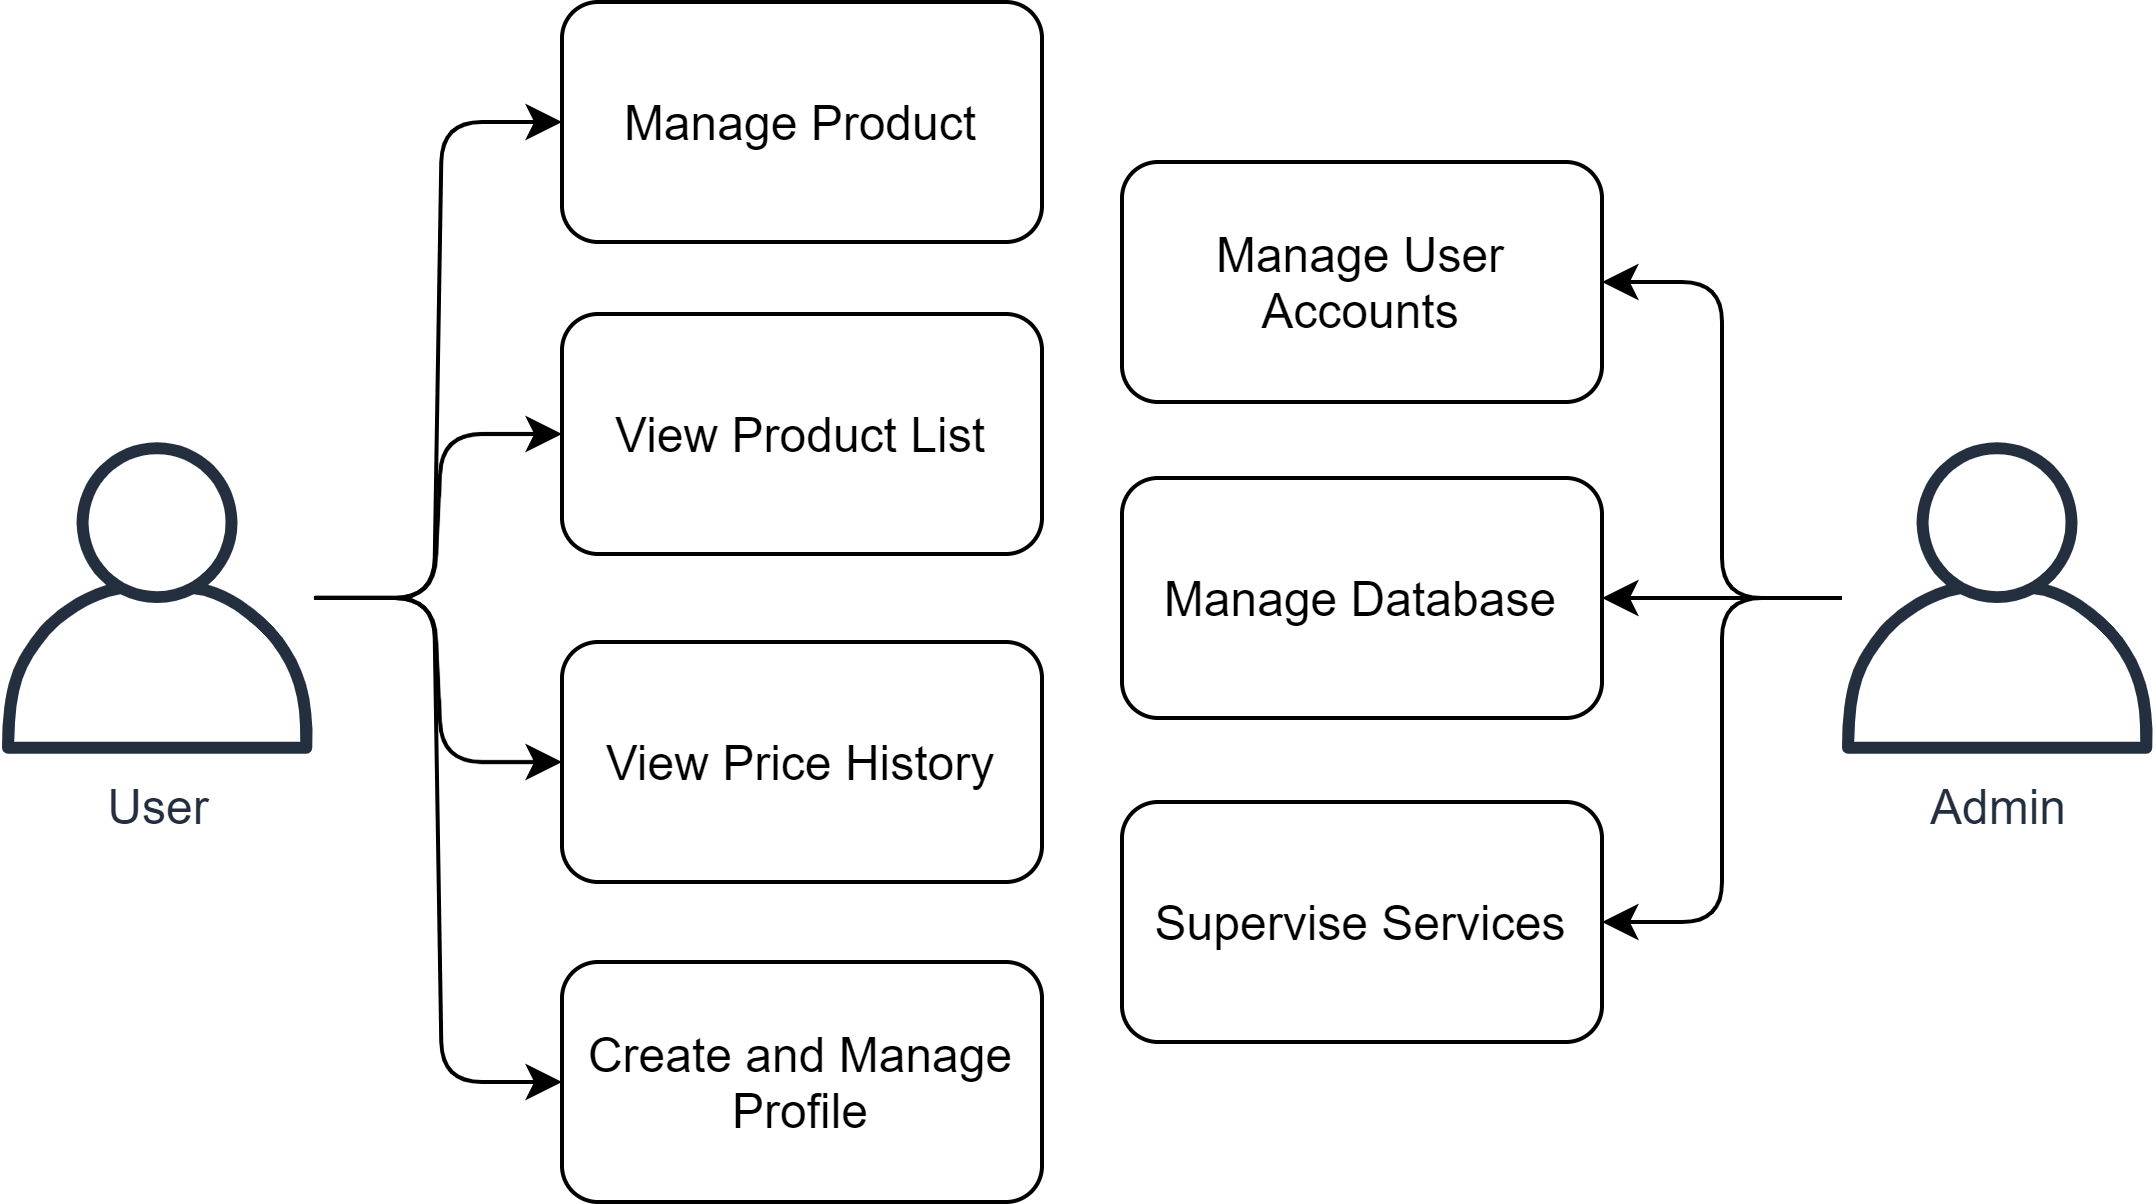
\includegraphics[scale=1.2]{figures/images/general_use_case.png}
    \caption{Use Case diagram}
    \label{fig:general_use_case}
\end{figure}
\section{Felhasználói Követelmények}

Amint a \ref{fig:general_use_case} ábra mutatja, a rendszer használata során két alapvető szerepet lehet elkülöníteni, az egyik a tulajdonképpeni felhasználó, aki használja a rendszert, igénybe veszi a szolgáltatást, a másik pedig egy adminisztrátor szerepkört betöltő személy. A következőkben e két szerepet betöltő személy követelményei lesznek bemutatva.


\textbf{Felhasználó:}
\begin{itemize}
    \item Menedzselni tudja a profilját, vagyis regisztrálni, bejelentkezni tud, illetve, lehetősége van a jelszavának módosítására vagy adott esetben a profil törlésére
    \item Megtekintheti a termékeket tartalmazó listáját
    \item Kezelheti a termékeket tartalmazó listáját, vagyis új termékeket adhat hozzá, esetleg törölhet belőle
    \item Részletes reprezentálást kaphat a követett termékek árának változásáról, a követes pillanatától kezdődően
    \item Weboldal melyen követni szeretné a termékeket: Emag
\end{itemize}

\textbf{Adminisztrátor:}
\begin{itemize}
    \item Kezeli a felhasználók fiókjait, az azokkal közbejövő problémákat
    \item Kezeli az adatbázist
    \item Felügyeli a rendszerek helyes működését, karbantartja a rendszert
\end{itemize}

% A felhasználónak mindenekelőtt be kell tudnia jelentkezni, ahhoz, hogy elérje a terméklistáját, ez azért fontos, mivel eszköz váltás esetén nem szeretnénk elveszíteni az addig követett termékeket. A bejelentkezéshez szükséges adatok a regisztrációkor megadott email cím, illetve jelszó. A felhasználó jelszava titkosítva kell legyen tárolás előtt, valamint lehetősége kell legyen igényelni annak változtatását.

% Abban az esetben, ha a felhasználó nincs regisztrálva, természetesen ez a funkcionalitás is rendelkezésére áll. A regisztrációhoz szükséges egy érvényes e-mail cím, valamint jelszó megadása. Sikeres regisztrálás esetén a felhasználó vissza kerül a bejelentkező ablakra, ahol be tud lépni, azzal a feltétellel, hogy az automatikusan küldött levél által visszaigazolta email címét. A bejelentkezést követően a felhasználó a főoldalra kerül, ahol a követett termékek listáját tekintheti meg, valamint ezen az oldalon lehetősége van a új termékeket hozzá adni a listához.

% A felhasználó egy grafikonon tekintheti meg az adott termék árának változását a hozzáadás napjától az aktuális dátumig, lásd \ref{fig:chart_example} ábra. Ha a felhasználó úgy dönt, hogy érdekli a termék, lehetősége kell legyen megnyitni az adott oldalt. Amennyiben a felhasználó már nem érdekelt a termék követesében, törölheti az adott terméket, igy az többet nem fog szerepelni a listájában.

% \begin{figure}[H]
%     \centering
%     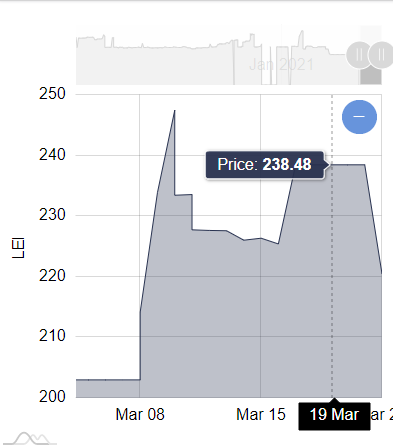
\includegraphics[scale=1]{figures/images/extension_chart_ss.png}
%     \caption{Az ár változását ábrázoló diagram}
%     \label{fig:chart_example}
% \end{figure}

% A felhasználónak rendelkezésére kell bocsájtani egy információs részt, amely röviden leírja az alkalmazás használatát, illetve tartalmazza az általa támogatott weboldalak listáját. Továbbá, hasonló módon, a fiókjával kapcsolatos információkat és funkciókat is el kell érnie. Itt tekintheti meg a felhasználó, hogy milyen email címmel jelentkezett be, törölheti a fiókját, illetve kijelentkezhet az alkalmazásból.

% Amint a \ref{fig:general_use_case} ábra is mutatja, a rendszernek szüksége van egy adminisztrátor szerepkört betöltő felhasználóra is, aki figyelemmel tudja követni a rendszerek helyes működését, illetve javító munkálatokat tud végezni úgy az adatbázis, mint a termékeket kezelő szoftver esetében is.

\section{Rendszer Követelmények}

\subsection{Funkcionális követelmények}

A rendszernek mindenek elött, egy bejelentkezési, illetve, regisztrálási felülettel kell rendelkeznie. Regisztrálás után, a felhasználónak egy ellenőrző email-t kell kapnia, amivel igazolja, hogy ő a cím tulajdonosa. A bejelentkezés nem lehetséges, abban az esetben, ha a felhasználó nem igazolta vissza az előbb említett email-ben a címét. A cím igazolása egy linkre való kattintással történik.

A felhasználónak lehetősége van a jelszavának módosítására melyet a bejelentkezési felületről ér el. Miután a felhasználó beírta az email címét, egy levelet fog kapni az adott címre, amelyen keresztül új jelszót tud beállítani.

Bejelentkezést követően, a felhasználó egy felületet lát, melyen bizonyos műveleteket végezhet. Megtekintheti a profiljához tartozó email címét, valamint törölheti a felhasználóját. Ugyanakkor, lehetősége van kijelentkezni az alkalmazásából melynek hatására újra a bejelentkezési oldalra kerül.

Ugyancsak a főoldalról a felhasználónak lehetősége van az alkalmazás használatával kapcsolatos információk megtekintésére mely tartalmaz egy listát is. A lista bizonyos weboldalakat tartalmaz, melyeket kiválasztva, az alkalmazás átirányít az adott elem oldalára.

A felhasználónak lehetősége van termékeket hozzáadni és kitörölni a listájából, valamint görgetni a lista tartalmában. Amennyiben frissíteni szeretné a lista tartalmát, ez úgy lehetséges, hogy a lista tetején tartózkodva, annak tartalmát megpróbálja görgetni (swipe down). A terméklistában egy elemet kiválasztva, részletes reprezentációt kap az adott elem tárolt adatairól, mint például aktuális ár, annak időbeli változása, hozzáadás időpontja, termék megnevezése.

Egy listaelem tartalmazza a termék megnevezését, aktuális árát, illetve egy képet róla. A termék ára mellett egy nyíl található, mely azt jelzi a felhasználó számára, hogy az aktuális ár hogyan változott a korábbi ellenőrzéshez kepést. A termék árának csökkenését, egy lefele irányuló, a növekedését egy felfele irányuló, amennyiben pedig az nem változott, egy vízszintesen irányított nyíl jelzi. Ezeket a változásokat színekkel is kell jelezni, mely az árra és az előbb említett nyílra hat ki. Csökkenés esetén zöld, növekvés esetén piros, valamint, ha változatlan, akkor fehér vagy fekete színnel kell jelölni ezeket.

Amennyiben egy új termék került hozzáadásra vagy a termék törlése következett be, a rendszernek ezt fel kell ismernie és elvégeznie a szükséges lepéseket annak érdekében, hogy a felhasználó számára mindig a legfrissebb adatok legyenek láthatóak. Amikor egy új terméket adott hozzá a felhasználó, a rendszer azonnal lekéri az adott webcím kódját, amiból kiveszi a szükséges adatokat, megnevezés, fénykép, aktuális ár, majd ezeket feltolti az adatbázisba az adott felhasználóhoz csatolva.

A rendszer back-end részének, mely a termékek hozzáadásáért és az adatbázis periodikus frissítéséért felelős, autonóm módon kell működni, minimális beavatkozással. Amikor egy felhasználó hozzá szeretne adni egy terméket, a rendszer azonnal reagáljon erre a kérésre.

\subsection{Nem-Funkcionális követelmények}

A rendszer backend része, mely a felhasználok által hozzáadott teremkék árainak ellenőrzését, frissítését, hozzáadását végzi, megszakítás nélkül kell működnie, napszaktól függetlenül. A rendszerre fel kell legyen telepítve a Python 3.8.0 vagy ennél frissebb verzió. Létfontosságú, hogy egy stabil Internet kapcsolattal rendelkezzen, vagyis a kapcsolatban ne legyenek megszakítások, valamint a fel-letöltési sebesség ne csökkenjen 10 Mb/s alá, annak érdekében, hogy megfelelő sebességgel lehessen az adatfeldolgozást, valamint az adatok adatbázisba való fel-, letöltését elvégezni. Amennyiben a kapcsolat megszakad, a rendszer azonnal próbáljon újrakapcsolódni, mindaddig amig ez a művelet nem sikers.

A rendszer vizuális felülete két alapvető platformon kell elérhető legyen. Az egyik egy böngésző kiegészítő, mely bármilyen Chromium alapú böngészőre telepíthető, asztali, valamint hordozható számítógépek eseteben is, legalább 58-as verziójú Chrome-ot tamogatva. Természetesen ebben az esetben is elengedhetetlen az Internethez való csatlakozás.

A másik egy telefonos alkalmazás, mely Android operációs rendszerrel felszerelt készülékeken legyen elérhető. Az alkalmazásnak legalább 7.0 verziójú Androiddal felszerelt telefonokon kell működnie, mely rendelkezik stabil Internetkapcsolattal. Rendelkeznie kell Light illetve Dark móddal is, melyek közötti váltást automatikusan végzi, az operációs rendszer beállításaihoz igazodva. A felhasználó számára, a követett termékeit egy görgethető listában kell megjeleníteni.

Úgy a telefonos alkalmazás, mint a böngésző kiegészítő esetében szükség van Internet használati jogosultságra. Továbbá, a kiegészítő eseteben még szükségesek a következő jogosultságok: "storage", "unlimitedStorage", "tabs", "activeTab", "<all\textunderscore urls>".

A rendszer a Firebase által biztosított Realtime Database nevű adatbázist kell használnia az adatok tárolására. A felhasználó bejelentkezését és a fiókjához tartozó műveleteket szintén a Firebase által biztosított Authentication szolgáltatás végezze, mivel ez biztonságos módon tárolja a szükséges információkat, ugyanakkor, a jelszavakat titkosítva kezeli. Továbbá, ezen keresztül lehessen új jelszót beállítani, a felhasználót törölni, ugyanakkor a regisztrálás után szükséges email visszaigazolása is ezen a szolgáltatáson keresztül történjen, mivel ezekre egyszerűen használható, ugyanakkor hatékony és biztonságos megoldást nyújt.

Az alkalmazás könnyen használható kell legyen, a felhasználónak minden funkciót három kattintáson belül el kell érnie. Amikor a felhasználó egy új terméket szeretne hozzáadni a listájához, ne keljen több mint 5 másodpercet várnia ahhoz, hogy az új termék megjelenjen a listájában. 

A rendszernek meg kell felelnie az érvényben lévő Európai, valamint Romániai törvényeknek melyek az adatok kinyerésére érvényesek. Továbbá, eleget kell tegyenek a bányászott weboldalak előírásainak is, melyek az adatok felhasználására és kinyerésére vonatkoznak.
